\documentclass[11pt]{article}
%% preamble.tex
%% this should be included with a command like
%% %% preamble.tex
%% this should be included with a command like
%% %% preamble.tex
%% this should be included with a command like
%% \input{p}

\usepackage{amsfonts}
\usepackage{amsthm}
\usepackage{latexsym}
\usepackage{amsmath}
%\usepackage{newalg}
\usepackage{amssymb}
\usepackage{latexsym}
\usepackage{subfigure}
\usepackage{graphicx}
\usepackage{wasysym}
\usepackage{booktabs}
\usepackage{hyperref}
\usepackage{mathtools}
\usepackage[makeroom]{cancel}
\usepackage{enumerate}
\usepackage{framed}
\usepackage{tikz}
\usepackage{mdframed}
\usepackage{algorithm}
\usepackage[noend]{algpseudocode}

% THEOREMS AND DEFINITIONS
\newcommand{\sk}{s}
\newtheorem{theorem}{Theorem}
\newtheorem{lesson}{Lesson}
\newtheorem{proposition}{Proposition}
\newtheorem{lemma}{Lemma}
\newtheorem{corollary}{Corollary}
\newtheorem{fact}{Fact}
\newtheorem*{claim}{Claim}
%\theoremstyle{definition}
\newtheorem{definition}{Definition}
\newtheorem{assumption}{Assumption}
\theoremstyle{remark}
\newtheorem{example}{Example}
\newtheorem*{remark}{Remark}

% DEFINITION command
%\newcounter{definitionCount}
%\setcounter{definitionCount}{0}
%\newcommand{\definition}[1]{
%\addtocounter{definitionCount}{1}
%\begin{mdframed}[backgroundcolor=gray!3,roundcorner=4pt]\textbf{ Definition \arabic{definitionCount}:} #1
%\end{mdframed}}

%==============================================================================
% Macros.
%==============================================================================
\newcommand{\new}[1]{{\em #1\/}}		% New term (set in italics).
\newcommand{\set}[1]{\{#1\}}			% Set (as in \set{1,2,3})
\newcommand{\setof}[2]{\{\,{#1}|~{#2}\,\}}	% Set (as in \setof{x}{x > 0})
\newcommand{\C}{\mathbb{C}}	                % Complex numbers.
\newcommand{\Q}{\textsf{Q}}                     % Robinson Arithmetic
\newcommand{\R}{\textsf{R}}                     % The system R
\newcommand{\PA}{\textsf{PA}}                     % Peano Arithmetic
\newcommand{\LA}{$\mathcal{LA}$}			% Language of Arithmetic
\newcommand{\compl}[1]{\overline{#1}}		% Complement of ...     
\newcommand{\subproblem}[1]{\vspace{4 mm}\noindent {\bf (#1)} \\} % Subproblem (a), (b), etc...
\newcommand{\elem}[1]{\noindent{\bf #1}}	    % Proof element (Claim:, Proof:, etc.)
\newcommand{\spacerule}{\vspace{4mm}\hrule\vspace{4mm}} % Add an hrule with some space
\newcommand{\dmod}[2]{\left[ #1\ \text{mod}\ #2\right]} % My mod rule
\newcommand{\tab}[1]{\hspace{.2\textwidth}\rlap{#1}}

\newcommand{\ra}[1]{\renewcommand{\arraystretch}{#1}} % booktabs table cmd for spacing

% Misc lines and other formatting
\newcommand{\encircle}[1]{\tikz[baseline=(char.base)]\node[anchor=south west, draw,rectangle, rounded corners, inner sep=2pt, minimum size=6mm, text height=2mm](char){#1} ;} % Circled text
\newcommand{\midline}{
\begin{center}
\noindent\rule{4cm}{0.4pt}
\end{center}}

% GODEL NUMBERS
\newbox\gnBoxA
\newdimen\gnCornerHgt
\setbox\gnBoxA=\hbox{$\ulcorner$}
\global\gnCornerHgt=\ht\gnBoxA
\newdimen\gnArgHgt
\def\Godelnum #1{%
\setbox\gnBoxA=\hbox{$#1$}%
\gnArgHgt=\ht\gnBoxA%
\ifnum     \gnArgHgt<\gnCornerHgt \gnArgHgt=0pt%
\else \advance \gnArgHgt by -\gnCornerHgt%
\fi \raise\gnArgHgt\hbox{$\ulcorner$} \box\gnBoxA %
\raise\gnArgHgt\hbox{$\urcorner$}}

\DeclarePairedDelimiter{\ceil}{\lceil}{\rceil}
\DeclareSymbolFont{AMSb}{U}{msb}{m}{n}
\DeclareMathSymbol{\F}{\mathalpha}{AMSb}{"46}
\DeclareMathSymbol{\N}{\mathalpha}{AMSb}{"4E}
\DeclareMathSymbol{\X}{\mathalpha}{AMSb}{"58}
\DeclareMathSymbol{\Zz}{\mathalpha}{AMSb}{"5A}
\DeclareMathOperator*{\argmin}{arg\,min}
\DeclareMathOperator*{\argmax}{arg\,max}
\newcommand{\Z}[1]{{\ensuremath{\Zz_{#1}} }}
\newcommand{\Zs}[1]{\ensuremath{\Zz^{\ast}_{#1}}}
\newcommand{\Zn}{\Z{n}}
\newcommand{\Zns}{\Zs{n}}
\newcommand{\Zstar}[1]{\Zs{#1}}
\newcommand{\Zp}{{\Z{p}}}
\newcommand{\Zps}{\Zs{p}}
\newcommand{\Zqs}{\Zs{q}}
\newcommand{\Zq}{{\Z{q}}}
%\newcommand{\QR}{\mathop{\mathrm{QR}}\nolimits}
\newcommand{\ord}[1]{\mathop{\mathrm{ord}}({#1})}
\newcommand{\QR}[1]{\ensuremath{\textit{QR}_{#1}}}
\newcommand{\becomes}{:=}
\newcommand{\rem}[1]{\ensuremath{\ \operatorname{rem} #1}}  
\newcommand{\U}{{\mathcal{U}}}
\newcommand{\floor}[1]{\ensuremath{\lfloor{#1}\rfloor}}
\newcommand{\de}[1]{\ensuremath{\Delta{#1}}}
\newcommand{\js}[2]{\left( \frac{#1}{#2} \right)}
\newcommand{\E}[1]{{\bf E} \left[ #1 \right]}
\newcommand{\PR}[1]{{\bf Pr} \left[ #1 \right]}

\renewcommand{\QR}{{\mbox{QR}}}
\newcommand{\QNR}{{\mbox{QNR}}}
\newcommand{\crt}{{\mbox{CRT}}}
\newcommand{\rsa}{{\mbox{RSA}}}
\newcommand{\rsamod}{{\mbox{RSA-modulus}}}


\newcommand{\greq}[1]{\stackrel{#1}{=}}
\newcommand{\hash}{\ensuremath{\mathcal{H}}}
\newcommand{\negl}{{\tt neg}}
\newcommand{\cindist}{\stackrel{c}{\approx}}
\newcommand{\A}{{\mathcal{A}}}
\newcommand{\B}{{\mathcal{B}}}

\newcommand{\gen}{\mathit{Gen}}
\newcommand{\keygen}{\mathit{KeyGen}}
\newcommand{\RSA}{\mathit{RSA}}
\newcommand{\pk}{\mathit{pk}}
\newcommand{\PK}{\mathit{PK}}
\newcommand{\SK}{\mathit{SK}}
\newcommand{\sign}{\mathit{Sign}}
\newcommand{\verify}{\mathit{Verify}}

% Bew command
\newcommand{\Bew}[1]{\textsc{Bew}(\Godelnum{#1})}


\setlength{\oddsidemargin}{.25in}
\setlength{\evensidemargin}{.25in}
\setlength{\textwidth}{6in}
\setlength{\topmargin}{-0.4in}
\setlength{\textheight}{8.5in}

\newcommand{\handout}[5]{
   \renewcommand{\thepage}{#1-\arabic{page}}
   \noindent
   \begin{center}
   \framebox{
      \vbox{
    \hbox to 5.78in { {\bf PHIL1885: Incompleteness} \hfill #2 }
       \vspace{4mm}
       \hbox to 5.78in { {\Large \hfill #5  \hfill} }
       \vspace{2mm}
       \hbox to 5.78in { {\it #3 \hfill #4} }
      }
   }
   \end{center}
   \vspace*{4mm}
}

% REMOVES ALL INDENTATION
%\setlength{\parindent}{0pt}

\usepackage{parskip}

\newcommand{\ho}[4]{\handout{#1}{#2}{Instructor:
#3}{}{Handout #1: #4}}

\newcommand{\lnotes}[3]{\handout{#1}{#2}{Instructor:
#3}{}{Lecture #1}}

\newcommand{\solution}[1]{#1}
%\homework{number}{out}{due}{instructor}
\newcommand{\homework}[4]{\handout{HW #1}{#2}{Instructor: #4}{Due: #3}{Homework #1}}

%================================================
% problemset macros
%================================================
% count problems
%\newcounter{solutioncount}
%\setcounter{solutioncount}{0}
\newcommand{\problem}[1]{%
%\addtocounter{solutioncount}{1}%
\section*{Problem #1:}}

% lets you make alphabetical lists (at first-level of enumeration)
\newenvironment
  {alphabetize}{\renewcommand{\theenumi}{\alph{enumi}}\begin{enumerate}}
  {\end{enumerate}\renewcommand{\theenumi}{\arabic{enumi}}}

\usepackage{amsfonts}
\usepackage{amsthm}
\usepackage{latexsym}
\usepackage{amsmath}
%\usepackage{newalg}
\usepackage{amssymb}
\usepackage{latexsym}
\usepackage{subfigure}
\usepackage{graphicx}
\usepackage{wasysym}
\usepackage{booktabs}
\usepackage{hyperref}
\usepackage{mathtools}
\usepackage[makeroom]{cancel}
\usepackage{enumerate}
\usepackage{framed}
\usepackage{tikz}
\usepackage{mdframed}
\usepackage{algorithm}
\usepackage[noend]{algpseudocode}

% THEOREMS AND DEFINITIONS
\newcommand{\sk}{s}
\newtheorem{theorem}{Theorem}
\newtheorem{lesson}{Lesson}
\newtheorem{proposition}{Proposition}
\newtheorem{lemma}{Lemma}
\newtheorem{corollary}{Corollary}
\newtheorem{fact}{Fact}
\newtheorem*{claim}{Claim}
%\theoremstyle{definition}
\newtheorem{definition}{Definition}
\newtheorem{assumption}{Assumption}
\theoremstyle{remark}
\newtheorem{example}{Example}
\newtheorem*{remark}{Remark}

% DEFINITION command
%\newcounter{definitionCount}
%\setcounter{definitionCount}{0}
%\newcommand{\definition}[1]{
%\addtocounter{definitionCount}{1}
%\begin{mdframed}[backgroundcolor=gray!3,roundcorner=4pt]\textbf{ Definition \arabic{definitionCount}:} #1
%\end{mdframed}}

%==============================================================================
% Macros.
%==============================================================================
\newcommand{\new}[1]{{\em #1\/}}		% New term (set in italics).
\newcommand{\set}[1]{\{#1\}}			% Set (as in \set{1,2,3})
\newcommand{\setof}[2]{\{\,{#1}|~{#2}\,\}}	% Set (as in \setof{x}{x > 0})
\newcommand{\C}{\mathbb{C}}	                % Complex numbers.
\newcommand{\Q}{\textsf{Q}}                     % Robinson Arithmetic
\newcommand{\R}{\textsf{R}}                     % The system R
\newcommand{\PA}{\textsf{PA}}                     % Peano Arithmetic
\newcommand{\LA}{$\mathcal{LA}$}			% Language of Arithmetic
\newcommand{\compl}[1]{\overline{#1}}		% Complement of ...     
\newcommand{\subproblem}[1]{\vspace{4 mm}\noindent {\bf (#1)} \\} % Subproblem (a), (b), etc...
\newcommand{\elem}[1]{\noindent{\bf #1}}	    % Proof element (Claim:, Proof:, etc.)
\newcommand{\spacerule}{\vspace{4mm}\hrule\vspace{4mm}} % Add an hrule with some space
\newcommand{\dmod}[2]{\left[ #1\ \text{mod}\ #2\right]} % My mod rule
\newcommand{\tab}[1]{\hspace{.2\textwidth}\rlap{#1}}

\newcommand{\ra}[1]{\renewcommand{\arraystretch}{#1}} % booktabs table cmd for spacing

% Misc lines and other formatting
\newcommand{\encircle}[1]{\tikz[baseline=(char.base)]\node[anchor=south west, draw,rectangle, rounded corners, inner sep=2pt, minimum size=6mm, text height=2mm](char){#1} ;} % Circled text
\newcommand{\midline}{
\begin{center}
\noindent\rule{4cm}{0.4pt}
\end{center}}

% GODEL NUMBERS
\newbox\gnBoxA
\newdimen\gnCornerHgt
\setbox\gnBoxA=\hbox{$\ulcorner$}
\global\gnCornerHgt=\ht\gnBoxA
\newdimen\gnArgHgt
\def\Godelnum #1{%
\setbox\gnBoxA=\hbox{$#1$}%
\gnArgHgt=\ht\gnBoxA%
\ifnum     \gnArgHgt<\gnCornerHgt \gnArgHgt=0pt%
\else \advance \gnArgHgt by -\gnCornerHgt%
\fi \raise\gnArgHgt\hbox{$\ulcorner$} \box\gnBoxA %
\raise\gnArgHgt\hbox{$\urcorner$}}

\DeclarePairedDelimiter{\ceil}{\lceil}{\rceil}
\DeclareSymbolFont{AMSb}{U}{msb}{m}{n}
\DeclareMathSymbol{\F}{\mathalpha}{AMSb}{"46}
\DeclareMathSymbol{\N}{\mathalpha}{AMSb}{"4E}
\DeclareMathSymbol{\X}{\mathalpha}{AMSb}{"58}
\DeclareMathSymbol{\Zz}{\mathalpha}{AMSb}{"5A}
\DeclareMathOperator*{\argmin}{arg\,min}
\DeclareMathOperator*{\argmax}{arg\,max}
\newcommand{\Z}[1]{{\ensuremath{\Zz_{#1}} }}
\newcommand{\Zs}[1]{\ensuremath{\Zz^{\ast}_{#1}}}
\newcommand{\Zn}{\Z{n}}
\newcommand{\Zns}{\Zs{n}}
\newcommand{\Zstar}[1]{\Zs{#1}}
\newcommand{\Zp}{{\Z{p}}}
\newcommand{\Zps}{\Zs{p}}
\newcommand{\Zqs}{\Zs{q}}
\newcommand{\Zq}{{\Z{q}}}
%\newcommand{\QR}{\mathop{\mathrm{QR}}\nolimits}
\newcommand{\ord}[1]{\mathop{\mathrm{ord}}({#1})}
\newcommand{\QR}[1]{\ensuremath{\textit{QR}_{#1}}}
\newcommand{\becomes}{:=}
\newcommand{\rem}[1]{\ensuremath{\ \operatorname{rem} #1}}  
\newcommand{\U}{{\mathcal{U}}}
\newcommand{\floor}[1]{\ensuremath{\lfloor{#1}\rfloor}}
\newcommand{\de}[1]{\ensuremath{\Delta{#1}}}
\newcommand{\js}[2]{\left( \frac{#1}{#2} \right)}
\newcommand{\E}[1]{{\bf E} \left[ #1 \right]}
\newcommand{\PR}[1]{{\bf Pr} \left[ #1 \right]}

\renewcommand{\QR}{{\mbox{QR}}}
\newcommand{\QNR}{{\mbox{QNR}}}
\newcommand{\crt}{{\mbox{CRT}}}
\newcommand{\rsa}{{\mbox{RSA}}}
\newcommand{\rsamod}{{\mbox{RSA-modulus}}}


\newcommand{\greq}[1]{\stackrel{#1}{=}}
\newcommand{\hash}{\ensuremath{\mathcal{H}}}
\newcommand{\negl}{{\tt neg}}
\newcommand{\cindist}{\stackrel{c}{\approx}}
\newcommand{\A}{{\mathcal{A}}}
\newcommand{\B}{{\mathcal{B}}}

\newcommand{\gen}{\mathit{Gen}}
\newcommand{\keygen}{\mathit{KeyGen}}
\newcommand{\RSA}{\mathit{RSA}}
\newcommand{\pk}{\mathit{pk}}
\newcommand{\PK}{\mathit{PK}}
\newcommand{\SK}{\mathit{SK}}
\newcommand{\sign}{\mathit{Sign}}
\newcommand{\verify}{\mathit{Verify}}

% Bew command
\newcommand{\Bew}[1]{\textsc{Bew}(\Godelnum{#1})}


\setlength{\oddsidemargin}{.25in}
\setlength{\evensidemargin}{.25in}
\setlength{\textwidth}{6in}
\setlength{\topmargin}{-0.4in}
\setlength{\textheight}{8.5in}

\newcommand{\handout}[5]{
   \renewcommand{\thepage}{#1-\arabic{page}}
   \noindent
   \begin{center}
   \framebox{
      \vbox{
    \hbox to 5.78in { {\bf PHIL1885: Incompleteness} \hfill #2 }
       \vspace{4mm}
       \hbox to 5.78in { {\Large \hfill #5  \hfill} }
       \vspace{2mm}
       \hbox to 5.78in { {\it #3 \hfill #4} }
      }
   }
   \end{center}
   \vspace*{4mm}
}

% REMOVES ALL INDENTATION
%\setlength{\parindent}{0pt}

\usepackage{parskip}

\newcommand{\ho}[4]{\handout{#1}{#2}{Instructor:
#3}{}{Handout #1: #4}}

\newcommand{\lnotes}[3]{\handout{#1}{#2}{Instructor:
#3}{}{Lecture #1}}

\newcommand{\solution}[1]{#1}
%\homework{number}{out}{due}{instructor}
\newcommand{\homework}[4]{\handout{HW #1}{#2}{Instructor: #4}{Due: #3}{Homework #1}}

%================================================
% problemset macros
%================================================
% count problems
%\newcounter{solutioncount}
%\setcounter{solutioncount}{0}
\newcommand{\problem}[1]{%
%\addtocounter{solutioncount}{1}%
\section*{Problem #1:}}

% lets you make alphabetical lists (at first-level of enumeration)
\newenvironment
  {alphabetize}{\renewcommand{\theenumi}{\alph{enumi}}\begin{enumerate}}
  {\end{enumerate}\renewcommand{\theenumi}{\arabic{enumi}}}

\usepackage{amsfonts}
\usepackage{amsthm}
\usepackage{latexsym}
\usepackage{amsmath}
%\usepackage{newalg}
\usepackage{amssymb}
\usepackage{latexsym}
\usepackage{subfigure}
\usepackage{graphicx}
\usepackage{wasysym}
\usepackage{booktabs}
\usepackage{hyperref}
\usepackage{mathtools}
\usepackage[makeroom]{cancel}
\usepackage{enumerate}
\usepackage{framed}
\usepackage{tikz}
\usepackage{mdframed}
\usepackage{algorithm}
\usepackage[noend]{algpseudocode}

% THEOREMS AND DEFINITIONS
\newcommand{\sk}{s}
\newtheorem{theorem}{Theorem}
\newtheorem{lesson}{Lesson}
\newtheorem{proposition}{Proposition}
\newtheorem{lemma}{Lemma}
\newtheorem{corollary}{Corollary}
\newtheorem{fact}{Fact}
\newtheorem*{claim}{Claim}
%\theoremstyle{definition}
\newtheorem{definition}{Definition}
\newtheorem{assumption}{Assumption}
\theoremstyle{remark}
\newtheorem{example}{Example}
\newtheorem*{remark}{Remark}

% DEFINITION command
%\newcounter{definitionCount}
%\setcounter{definitionCount}{0}
%\newcommand{\definition}[1]{
%\addtocounter{definitionCount}{1}
%\begin{mdframed}[backgroundcolor=gray!3,roundcorner=4pt]\textbf{ Definition \arabic{definitionCount}:} #1
%\end{mdframed}}

%==============================================================================
% Macros.
%==============================================================================
\newcommand{\new}[1]{{\em #1\/}}		% New term (set in italics).
\newcommand{\set}[1]{\{#1\}}			% Set (as in \set{1,2,3})
\newcommand{\setof}[2]{\{\,{#1}|~{#2}\,\}}	% Set (as in \setof{x}{x > 0})
\newcommand{\C}{\mathbb{C}}	                % Complex numbers.
\newcommand{\Q}{\textsf{Q}}                     % Robinson Arithmetic
\newcommand{\R}{\textsf{R}}                     % The system R
\newcommand{\PA}{\textsf{PA}}                     % Peano Arithmetic
\newcommand{\LA}{$\mathcal{LA}$}			% Language of Arithmetic
\newcommand{\compl}[1]{\overline{#1}}		% Complement of ...     
\newcommand{\subproblem}[1]{\vspace{4 mm}\noindent {\bf (#1)} \\} % Subproblem (a), (b), etc...
\newcommand{\elem}[1]{\noindent{\bf #1}}	    % Proof element (Claim:, Proof:, etc.)
\newcommand{\spacerule}{\vspace{4mm}\hrule\vspace{4mm}} % Add an hrule with some space
\newcommand{\dmod}[2]{\left[ #1\ \text{mod}\ #2\right]} % My mod rule
\newcommand{\tab}[1]{\hspace{.2\textwidth}\rlap{#1}}

\newcommand{\ra}[1]{\renewcommand{\arraystretch}{#1}} % booktabs table cmd for spacing

% Misc lines and other formatting
\newcommand{\encircle}[1]{\tikz[baseline=(char.base)]\node[anchor=south west, draw,rectangle, rounded corners, inner sep=2pt, minimum size=6mm, text height=2mm](char){#1} ;} % Circled text
\newcommand{\midline}{
\begin{center}
\noindent\rule{4cm}{0.4pt}
\end{center}}

% GODEL NUMBERS
\newbox\gnBoxA
\newdimen\gnCornerHgt
\setbox\gnBoxA=\hbox{$\ulcorner$}
\global\gnCornerHgt=\ht\gnBoxA
\newdimen\gnArgHgt
\def\Godelnum #1{%
\setbox\gnBoxA=\hbox{$#1$}%
\gnArgHgt=\ht\gnBoxA%
\ifnum     \gnArgHgt<\gnCornerHgt \gnArgHgt=0pt%
\else \advance \gnArgHgt by -\gnCornerHgt%
\fi \raise\gnArgHgt\hbox{$\ulcorner$} \box\gnBoxA %
\raise\gnArgHgt\hbox{$\urcorner$}}

\DeclarePairedDelimiter{\ceil}{\lceil}{\rceil}
\DeclareSymbolFont{AMSb}{U}{msb}{m}{n}
\DeclareMathSymbol{\F}{\mathalpha}{AMSb}{"46}
\DeclareMathSymbol{\N}{\mathalpha}{AMSb}{"4E}
\DeclareMathSymbol{\X}{\mathalpha}{AMSb}{"58}
\DeclareMathSymbol{\Zz}{\mathalpha}{AMSb}{"5A}
\DeclareMathOperator*{\argmin}{arg\,min}
\DeclareMathOperator*{\argmax}{arg\,max}
\newcommand{\Z}[1]{{\ensuremath{\Zz_{#1}} }}
\newcommand{\Zs}[1]{\ensuremath{\Zz^{\ast}_{#1}}}
\newcommand{\Zn}{\Z{n}}
\newcommand{\Zns}{\Zs{n}}
\newcommand{\Zstar}[1]{\Zs{#1}}
\newcommand{\Zp}{{\Z{p}}}
\newcommand{\Zps}{\Zs{p}}
\newcommand{\Zqs}{\Zs{q}}
\newcommand{\Zq}{{\Z{q}}}
%\newcommand{\QR}{\mathop{\mathrm{QR}}\nolimits}
\newcommand{\ord}[1]{\mathop{\mathrm{ord}}({#1})}
\newcommand{\QR}[1]{\ensuremath{\textit{QR}_{#1}}}
\newcommand{\becomes}{:=}
\newcommand{\rem}[1]{\ensuremath{\ \operatorname{rem} #1}}  
\newcommand{\U}{{\mathcal{U}}}
\newcommand{\floor}[1]{\ensuremath{\lfloor{#1}\rfloor}}
\newcommand{\de}[1]{\ensuremath{\Delta{#1}}}
\newcommand{\js}[2]{\left( \frac{#1}{#2} \right)}
\newcommand{\E}[1]{{\bf E} \left[ #1 \right]}
\newcommand{\PR}[1]{{\bf Pr} \left[ #1 \right]}

\renewcommand{\QR}{{\mbox{QR}}}
\newcommand{\QNR}{{\mbox{QNR}}}
\newcommand{\crt}{{\mbox{CRT}}}
\newcommand{\rsa}{{\mbox{RSA}}}
\newcommand{\rsamod}{{\mbox{RSA-modulus}}}


\newcommand{\greq}[1]{\stackrel{#1}{=}}
\newcommand{\hash}{\ensuremath{\mathcal{H}}}
\newcommand{\negl}{{\tt neg}}
\newcommand{\cindist}{\stackrel{c}{\approx}}
\newcommand{\A}{{\mathcal{A}}}
\newcommand{\B}{{\mathcal{B}}}

\newcommand{\gen}{\mathit{Gen}}
\newcommand{\keygen}{\mathit{KeyGen}}
\newcommand{\RSA}{\mathit{RSA}}
\newcommand{\pk}{\mathit{pk}}
\newcommand{\PK}{\mathit{PK}}
\newcommand{\SK}{\mathit{SK}}
\newcommand{\sign}{\mathit{Sign}}
\newcommand{\verify}{\mathit{Verify}}

% Bew command
\newcommand{\Bew}[1]{\textsc{Bew}(\Godelnum{#1})}


\setlength{\oddsidemargin}{.25in}
\setlength{\evensidemargin}{.25in}
\setlength{\textwidth}{6in}
\setlength{\topmargin}{-0.4in}
\setlength{\textheight}{8.5in}

\newcommand{\handout}[5]{
   \renewcommand{\thepage}{#1-\arabic{page}}
   \noindent
   \begin{center}
   \framebox{
      \vbox{
    \hbox to 5.78in { {\bf PHIL1885: Incompleteness} \hfill #2 }
       \vspace{4mm}
       \hbox to 5.78in { {\Large \hfill #5  \hfill} }
       \vspace{2mm}
       \hbox to 5.78in { {\it #3 \hfill #4} }
      }
   }
   \end{center}
   \vspace*{4mm}
}

% REMOVES ALL INDENTATION
%\setlength{\parindent}{0pt}

\usepackage{parskip}

\newcommand{\ho}[4]{\handout{#1}{#2}{Instructor:
#3}{}{Handout #1: #4}}

\newcommand{\lnotes}[3]{\handout{#1}{#2}{Instructor:
#3}{}{Lecture #1}}

\newcommand{\solution}[1]{#1}
%\homework{number}{out}{due}{instructor}
\newcommand{\homework}[4]{\handout{HW #1}{#2}{Instructor: #4}{Due: #3}{Homework #1}}

%================================================
% problemset macros
%================================================
% count problems
%\newcounter{solutioncount}
%\setcounter{solutioncount}{0}
\newcommand{\problem}[1]{%
%\addtocounter{solutioncount}{1}%
\section*{Problem #1:}}

% lets you make alphabetical lists (at first-level of enumeration)
\newenvironment
  {alphabetize}{\renewcommand{\theenumi}{\alph{enumi}}\begin{enumerate}}
  {\end{enumerate}\renewcommand{\theenumi}{\arabic{enumi}}}

\begin{document}

% TITLE PAGE
\begin{titlepage}
\begin{center}
\vfill
\textsc{\Large Brown University \\ Department of Computer Science}\\[1.5cm]

\vspace{55mm}

% Title
{ \huge \bfseries Learning to Plan in Complex  \\Stochastic Environments \\[0.9cm] }

% Author and supervisor
\noindent
\begin{minipage}[t]{0.4\textwidth}
\begin{flushleft} \large
\emph{Author:}\\
\textsc{David Abel}
\end{flushleft}
\end{minipage}%
\begin{minipage}[t]{0.4\textwidth}
\begin{flushright} \large
\emph{Supervisor:} \\
\textsc{Prof. Stefanie Tellex}
\end{flushright}
\end{minipage}

%\vspace{20mm}
%\textsc{\Large Sc.M Project Document}\\[0.5cm]

% Bottom of the page
\vfill
{\large May 2015}

\end{center}
\end{titlepage}
% End of Title Page

\newpage

% --- Abstract ---
\begin{abstract}
Probabilistic planning offers a powerful framework for general problem solving. Historically, probabilistic planning algorithms have contributed to a variety of critical technologies and application areas, ranging from conservation biology~\cite{possingham1997state} to self-driving cars~\cite{thrun2006stanley,montemerlo2008junior} to space exploration~\cite{bresina2005activity,backes1999automated,chien2000aspen}. Unfortunately, determining optimal solutions to probabilistic planning problems is known to be P-Complete~\cite{littman1995complexity} w.r.t. the problem complexity. This imposes a serious constraint the types of problems that may be solved in close to real time. In order to bolster our planning toolkit, we propose investigating methods of {\it learning to plan}. The critical insight is that problems that are too complex to solve efficiently often resemble much simpler problems for which optimal solutions may be computed. By extracting relevant characteristics of the simple problems' solutions, we develop algorithms to operate on the more complex problems that take advantage of prior knowledge of optimal behavior in similar tasks. In particular, we introduce {\it goal-based action priors}~\cite{abel2015goal}, that guide planing algorithms according to which actions are likely to be useful under different conditions. The priors are informed during a training stage in which simple, tractable tasks are solved, and the priors are then used to solve for optimal behavior in state spaces that are far more complex.
\end{abstract}

\newpage

% --- Acknowledgements ---
\section*{Acknowledgements}
This work would not have been possible without the help of my Advisor Professor Stefanie Tellex, whose constant guidance and support was essential for carrying out this research. Additionally, I would like to thank Ellis Hershkowitz, James MacGlashan, and Gabriel Barth-Maron for their critical contributions to this project, and for the many wonderful discussions that led to the central ideas introduced in this document. Lastly, I would like to thank the other members of the Humans to Robots laboratory, including Professor Michael Littman, David Whitney, Jeremy Joachim, Izaak Baker, Ryan Izant, Greg Yauney, Dilip Arumagum, Miles Eldon, Stephen Brawner, Nakul Goppalan, Kevin O'Farrell, Emily Wu, and John Oberlin.

% --- Table Of Contents ---
\newpage
\tableofcontents
\newpage

% --- Introduction ---
\section{Introduction}
\label{sec:introduction}

% Why is planning so baller?


\subsection{History}

\subsection{Learning to Plan}
An alternative approach is to {\it learn to plan}. In this sense, training  will slowly build up a set of skills, behaviors, and knowledge that dramatically simplify more complicated problems.
The tractability of planning problems depends critically on problem difficulty, though with the proper prior knowledge, challenging problems may be decomposed into tasks for which optimal behavior is known.

% What domains are we interested in?
\subsection{Domains}
%Domains of special interest are robotic navigation tasks that involve manipulation of the environment, such as pressing buttons, opening doors, and moving obstacles, as well as tackling more general problem solving strategies that include planning with 3D printers and programmable matter; suppose a robot could open a locked door by scanning the lock and printing the proper key. A composite robot-3D printer system would dramatically increase the scope of what robots can achieve. Robots could construct entire buildings on other planets, such as structures that offer protection from the harsh environments of foreign-atmospheres. The European Space Agency is already investigating using 3D printers to construct protective domes on the moon~\cite{ceccanti20103D,Cesaretti2014430} -- however, a 3D printer alone is stationary. The physical capabilities of a robot combined with the tool generation of a 3D printer offer many compelling advances in space exploration. If a part breaks on Mars, we need not send another entire mission to Mars, our robot can simply print another one. However, the space of printable objects is so massive that searching through possible futures is computationally intractable, calling for an advanced planning system that can reason over huge spaces, requiring succinct representations.



% --- Background ---
\section{Background}
\label{sec:background}

Why care about planning? Well, if we can formalize stuff in the right way, planning is a way of finding a sequence of actions for satisfying some condition.

Conditions can be formulated arbitrarily, so if we had a perfect planning algorithm, we could identify optimal strategies in the real world for arbitrary goals! That's pretty incredible.

In other words, planning has two pretty great properties: 1) it can represent just about any problem (at any level of abstraction), 2) advances in planning can then benefit a lot of stuff!

\subsection{Planning}

Planning is search! Older variants...

General Problem solver!

\subsection{Stochastic Planning}

Planning in the real world is a bad idea because of the stochasticity inherent in the world.

\subsection{Markov Decision Process}
{\definition A \textup{Markov Decision Process (MDP)} is a five-tuple: $\langle \mathcal{S},
\mathcal{A}, \mathcal{T}, \mathcal{R}, \gamma \rangle$, where:
\begin{itemize}
\item $\mathcal{S}$ is a finite set of states, also called the \textup{state space}.
\item $\mathcal{A}$ is a finite set of actions, also called the \textup{action space}.
\item $\mathcal{T}$ denotes $\mathcal{T}(s' \mid s,a)$, the
transition probability of an agent applying action $a \in \mathcal{A}$
in state $s \in \mathcal{S}$ and arriving in $s' \in \mathcal{S}$
\item $\mathcal{R} : \mathcal{S} \times \mathcal{A} \times \mathcal{S} \mapsto \mathbb{R}$ denotes the real valued reward received by the agent for
applying action $a$ in state $s$ and transitioning to state $s'$
\item $\gamma \in [0, 1)$ is a discount factor that defines how much the
  agent prefers immediate rewards over future rewards (the agent
  prefers to maximize immediate rewards as $\gamma$ decreases).
\end{itemize}}


\subsection{Solving Markov Decision Processes}



\subsubsection{Complexity}

{\theorem Optimal solutions for an MDP are $\mathcal{O}()$}

\subsubsection{Linear Programming}


\subsubsection{Value Iteration}

Algorithm Overview.

\subsubsection{Policy Iteration}

Algorithm Overview.

\subsubsection{Real Time Dynamic Programming}

Algorithm Overview.

\subsubsection{Bounded Real Time Dynamic Programming}



\subsection{Object Oriented Markov Decision Process}


An Object-Oriented Markov Decision Process (OO-MDP)~\cite{diuk08} efficiently represents the state
of an MDP through the use of objects and predicates. These predicates enable abstraction into agent space. \\

{\definition An \textup{Object-Oriented Markov Decision Process (OO-MDP)} is an eight tuple, $\langle \mathcal{C}, \textsc{Att}(c), \textsc{Dom}(a), \mathcal{O},
\mathcal{A}, \mathcal{T}, \mathcal{R}, \gamma \rangle$, where:

\begin{itemize}
\item $\mathcal{C}$ is a set of object classes.
\item $\textsc{Att}(c)$ is a function $\mathcal{C} \mapsto A$ that specifies the attributes associated with class $c \in \mathcal{C}$.
\item $\textsc{Dom}(a_i)$ is a function $A \mapsto [a,b]$, s.t. $\{x \in \mathbb{R} \mid a \leq x \leq b \}$, that specifies the space of possible values for an attribute $a_i$.
\item $\mathcal{O}$ is a collection of objects, $o \in \mathcal{O}$, where each object belongs to a class, $\mathcal{C}$. The \textup{state} of an object $o.state$ is a value assignment to all of its attributes.
\item $\mathcal{S}$ is a finite set of states, where a state is uniquely identified by $\bigcup_{o \in \mathcal{O}} o.state$/
\item $\mathcal{A}$ is a finite set of actions, also called the \textup{action space}.
\item $\mathcal{T}$ denotes $\mathcal{T}(s' \mid s,a)$, the
transition probability of an agent applying action $a \in \mathcal{A}$
in state $s \in \mathcal{S}$ and arriving in $s' \in \mathcal{S}$
\item $\mathcal{R} : \mathcal{S} \times \mathcal{A} \times \mathcal{S} \mapsto \mathbb{R}$ denotes the real valued reward received by the agent for
applying action $a$ in state $s$ and transitioning to state $s'$
\item $\gamma \in [0, 1)$ is a discount factor that defines how much the
  agent prefers immediate rewards over future rewards (the agent
  prefers to maximize immediate rewards as $\gamma$ decreases).
\end{itemize}}

An OO-MDP state is a collection of objects, $O = \{o_1, \ldots, o_o \}$.  Each object
$o_i$ belongs to a class, $c_j \in \{c_1, \ldots, c_c\}$. Every class
has a set of attributes, $Att(c) = \{c.a_1, \ldots, c.a_a \}$, each of
which has a domain, $Dom(c.a)$, of possible values. OO-MDPs enable
planners to use predicates over classes of objects. That is, the
OO-MDP definition also includes a set of predicates $\mathcal{P}$ that
operate on the state of objects to provide additional high-level
information about the MDP state.

Agent space stuff:
OO-MDP predicates provide state space independence. For a given planning domain, OO-MDP objects
often appear across tasks. Since predicates operate on collections
of objects, they generalize beyond specific state spaces within the domain.
For instance, in Minecraft, a predicate checking the contents of the agent's inventory
generalizes beyond any particular Minecraft task. We capitalize on this state space
independence by using OO-MDP predicates as features for action pruning.


\subsection{Hidden Parameter Markov Decision Process}

George's Paper! Neat framework for transfer learning.\cite{konidaris2014hidden}




\subsection{Transfer Learning}

\subsubsection{Agent Space}
\subsubsection{Options}


\subsubsection{Macroactions}



% --- OOP-MDPs ---
\section{OOP-MDPs}
\label{sec:oop_mdps}

Here we establish the basic notions required for a new model, the Object-Oriented Parameterized MDP, which naturally models families of related MDPs while maintaining the representational richness of the OO-MDP.

{\definition An \textup{Object Oriented Parameterized Markov Decision Process (OOP-MDP)} is a }

\subsection{Preliminaries}

\subsubsection{Definitions}
Idea: Domain is everything but R and S, but includes the object classes and stuff AND a parameter $\theta$.

Task: An assignment to the parameter vector theta (includes number of objects, attribute assignments, etc.)

{\definition A \textup{Problem Generator} is a randomized poly-time turing machine that samples from the disitribution associated with the OOP-MDP and returns a OO-MDP}

\subsubsection{Domains}

Minecraft, other?


% --- Action Pruning ---
\section{Action Pruning}
\label{sec:action_pruning}


% --- Goal-Based Action Priors
\section{Goal-Based Action Priors}
\label{sec:gbaps}

To address state-action space explosions in robotic planning tasks,
we augment an Object Oriented Markov Decision Process (OO-MDP) with a
specific type of action prior conditioned on the current state and an abstract goal description. This {\it goal-based action prior}
enables an agent to prune irrelevant actions on a
state-by-state basis according to the agent's current goal, focusing the agent on
the most promising parts of the state space.  
 
Goal-based action priors can be specified
by hand or learned through experience in related
problems, making them a concise, transferable, and learnable means of
representing useful planning knowledge. Our results demonstrate
that these priors provide dramatic improvements for a variety of
planning tasks compared to baselines in simulation, and are applicable
across different state spaces.  Moreover, while manually provided
priors outperform baselines on difficult problems, our approach
is able to learn goal-based action priors from experience on simple, tractable, 
training problems that yield even greater performance on the difficult problems
than manually provided priors.

We conduct experiments in
the game Minecraft, which has a very large state-action space, and on
a real-world robotic cooking assistant.  Figure~\ref{fig:example}
shows an example of two problems from the same domain in the game
Minecraft; the agent learns on simple randomly generated problems
(like the problem in the left image) and tests
on new harder problems from the same domain that it has never previously
encountered (like the problem in the right image). All associated code with this paper may be found at
http://h2r.cs.brown.edu/affordances.



\subsection{Approach}
Meat of GBAP paper.

Arbitrary model! We can use Naive bayes (results 1) or Log reg (results 2).

We define a {\it goal-based action prior} as knowledge added to a family of related
Markov Decision Processes (MDPs) from the same domain.  An MDP is a
five-tuple: $\langle \mathcal{S}, \mathcal{A}, \mathcal{T},
\mathcal{R}, \gamma \rangle$, where $\mathcal{S}$ is a state space;
$\mathcal{A}$ is the agent's set of actions; $\mathcal{T}$ denotes
$\mathcal{T}(s' \mid s,a)$, the transition probability of an agent
applying action $a \in \mathcal{A}$ in state $s \in \mathcal{S}$ and
arriving in $s' \in \mathcal{S}$; $\mathcal{R}(s,a,s')$ denotes the
reward received by the agent for applying action $a$ in state $s$ and
transitioning to state $s'$; and $\gamma \in [0, 1]$ is a discount
  factor that defines how much the agent prefers immediate rewards
  over future rewards (the agent prefers to maximize immediate rewards
  as $\gamma$ decreases). MDPs may also include terminal states
  that cause all action to cease once reached (such as in goal-directed
  tasks).


% -- Figure: Minecraft pic --
\begin{figure}[t]
\centering
\subfigure[Mine the gold and smelt it in the furnace]{
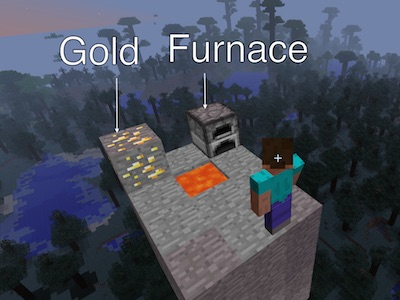
\includegraphics[width=0.3\linewidth]{figures/smelt_scaled_small.jpg}}
\subfigure[Dig down to the gold and mine it, avoiding lava.]{
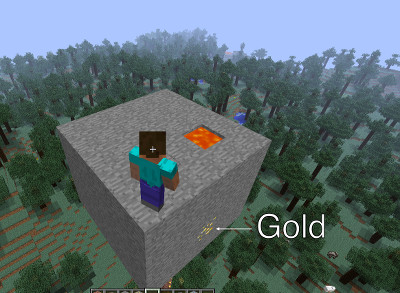
\includegraphics[width=0.3\linewidth]{figures/mining_labeled.jpg}}
\subfigure[Navigate to the goal location, avoiding lava.]{
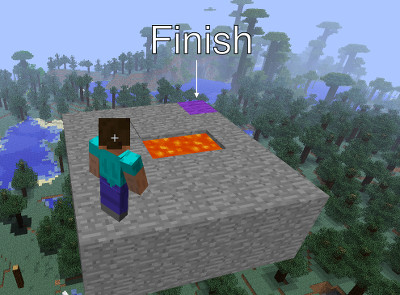
\includegraphics[width=0.3\linewidth]{figures/plane.jpg}}
  \caption{Three different problems from the Minecraft domain.}
  \label{fig:minecraft}
\end{figure}


% -- Subsection: Modeling the Optimal Actions --
\subsection{Modeling the Optimal Actions}

Our goal is to formalize planning knowledge that allows an agent to
avoid searching suboptimal actions in each state based on the agent's
current goal. We define the optimal action set, $\mathcal{A}^*$, for a
given state $s$ and goal $G$ as:
% -- Equation: Optimal Action Set --
\begin{equation}
\mathcal{A}^* = \left\{ a \mid Q^*_G(s,a) = V^*_G(s) \right\}, 
\label{eq:opt_act_set}
\end{equation}
where $Q^*_G(s,a)$ and $V^*_G(s)$ represent the optimal Q function and 
value function, respectively.

We aim to learn a probability distribution over the optimality of each action
for a given state ($s$) and goal ($G$). Thus, we want to infer a Bernoulli
distribution for each action's optimality:
% -- Equation: Master Equation --
\begin{equation}
\Pr(a_i \in \mathcal{A}^* \mid s, G)
\label{eq:master}
\end{equation}

\noindent for $i \in \{1, \ldots, |\mathcal{A}|\}$, where
$\mathcal{A}$ is the OO-MDP action space for the domain.

CRUCIAL: Agent Space:

The agent space representation of the problem is abstracted
into a set of $n$ paired preconditions and goals, $\{
(p_1, g_1) \ldots (p_{n}, g_{n}) \}$. We abbreviate each pair $(p_j,
g_j)$ to $\delta_j$ for simplicity. Each precondition $p \in
\mathcal{P}$ is a {\it predicate} in the set of predicates $\mathcal{P}$
defined by the OO-MDP domain, and $G$ is a {\it goal} which is a
predicate on states that is true if and only if a state is terminal. For example, a
predicate might be $nearTrench(agent)$ which is true when the agent is
standing near a trench.  In general a precondition is an arbitrary
logical expression of the state; in our experiments we used unary
predicates defined in the OO-MDP domain. A goal specifies the
sort of problem the agent is trying to solve, such as the agent
retrieving an object of a certain type from the environment, reaching
a particular location, or creating a new structure.  Depending on the
agent's current goal, the relevance of each action changes
dramatically.  We rewrite Equation~\ref{eq:master}:
% -- Equation: replace K --
\begin{equation}
\Pr(a_i \in \mathcal{A}^* \mid s, G) = \Pr(a_i \in \mathcal{A}^* \mid s, G, \delta_1 \ldots \delta_n).
\end{equation}

We introduce the indicator function $f$, which returns 1 if and only if the given $\delta$'s predicate is true in the provided state $s$, and $\delta$'s goal is entailed by the agent's current goal, $G$:
% -- Equation: function f defn --
\begin{equation}
f(\delta, s, G) = 
\begin{cases}
1& \delta.p(s) \wedge \delta.g(G) \\
0& \text{otherwise.}
\end{cases}
\label{eq:f_func_def}
\end{equation}

Evaluating $f$ for each $\delta_j$ given the current state and goal gives rise to a set of binary features,
$\phi_j = f(\delta_j, s, G)$, which we use to reformulate our probability distribution:
% -- Equation: Master Equation --
\begin{equation}
\Pr(a_i \in \mathcal{A}^*  \mid s, G, \delta_1 \ldots \delta_n) = \Pr(a_i \in \mathcal{A}^*  \mid \phi_1, \ldots, \phi_n)
\label{eq:feature_rep}
\end{equation}

Emphasize how crucial this equation is.

This distribution may be modeled in a number of ways, making this
approach quite flexible. 

{\bf Expert Model:} One model that can be easily specified by
an expert is an OR model.
In the OR model some subset of the features 
($\phi^i \subset \phi$) are
assumed to cause action $a_i$ to be optimal; as long as one of
the features is on, the probability that $a_i$ is optimal is one.
If none of the features are on, then the probability that $a_i$ is 
optimal is zero. More formally,
\begin{equation}
\Pr(a_i \in \mathcal{A}^*  \mid \phi_1, \ldots, \phi_n) = \phi_1^i \lor ... \lor \phi_m^i,
\end{equation}
where $m$ is the number of features that can cause $a_i$ to be optimal ($m = |\phi^i|$).

In practice, we do not expect such a distribution to be reflective of
reality; if it were, then no planning would be needed because a full
policy would have been specified. However, it does provide a
convenient way for a designer to provide conservative background
knowledge. Specifically, a designer can consider each precondition-goal
pair and specify the actions that could be optimal in that context, ruling
out actions that would be known to be irrelevant or dependent on other
state features being true.

Because the OR model is not expected to be reflective of
reality and because of other limitations (such as not allowing support
for an action to be provided when a feature is off), the model is not
practical for learning.

% Learned Priors
Learned priors have the potential to outperform
hand-coded priors by more flexibly adapting to the
features that predict optimal actions over a large training set.
We evaluate using two models, Naive Bayes and Logistic Regression.

\subsubsection{Naive Bayes}
An alternative more expressive model that does lend itself to learning is
Naive Bayes. We first factor using Bayes' rule, introducing a parameter vector $\theta_i$ of
feature weights:

% -- Equation: Bayes --
\begin{equation}
= \frac{\Pr(\phi_1, \ldots, \phi_{n}, \mid a_i \in \mathcal{A}^*, \theta_i) \Pr(a_i \in \mathcal{A}^* \mid \theta_i)}{\Pr(\phi_1, \ldots, \phi_{n} | \theta_i)}
\label{eq:bayes}
\end{equation}

Next we assume that each feature is conditionally independent of the others, given whether the action is optimal:
% -- Equation: Naive assumption and uniform prior--
\begin{equation}
= \frac{\prod_{j=1}^{n} \Pr(\phi_j \mid a_i \in \mathcal{A}^*, \theta_i) \Pr(a_i \in \mathcal{A}^* \mid \theta_i) }{\Pr(\phi_1, \ldots, \phi_{n} | \theta_i)}
\label{eq:final}
\end{equation}

Finally, we define the prior on the optimality of each action to be
the fraction of the time each action was optimal during training.


\subsubsection{Logistic Regression}

NEED MATH


% -- Subsection: Learning the Optimal Actions--
\subsection{Learning the Optimal Actions}
Using the above model allows us to learn goal-based action priors
through experience. We provide a set of
training worlds from the domain ($W$), for which the optimal policy,
$\pi$, may be tractably computed using existing planning methods.  We
compute model parameters using the small training worlds, and then
evaluate performance on a different set of much harder problems at
test time.  To compute model parameters using Naive Bayes, we compute
the maximum likelihood estimate of the parameter vector $\theta_i$ for
each action using the policy.

Under our Bernouli Naive Bayes model, we estimate the parameters
$\theta_{i,0} = \Pr(a_i)$ and $\theta_{i,j} = \Pr(\phi_j | a_i)$, for $j \in \{1, \ldots, n \}$, where the maximum likelihood estimates are:
\begin{align}
\theta_{i,0} &= \frac{C(a_i)}{C(a_i) + C(\bar{a_i})} \\
\theta_{i,j} &= \frac{C(\phi_j, a_i)}{C(a_i)}
\end{align}

Here, $C(a_i)$ is the number of observed occurrences where $a_i$ was optimal across all worlds $W$,
$C(\bar{a_i})$ is the number of observed occurrences where $a_i$ was not optimal,
and $C(\phi_j, a_i)$ is the number of occurrences where $\phi_j=1$ and $a_i$ was optimal.
We determined optimality using the synthesized policy for each training world, $\pi_w$. More formally:

\begin{align}
C(a_i) &= \sum_{w \in W} \sum_{s \in w} (a_i \in \pi_w(s)) \\
C(\bar{a_i}) &= \sum_{w \in W} \sum_{s \in w} (a_i \not \in \pi_w(s) ) \\
C(\phi_j, a_i) &= \sum_{w \in W} \sum_{s \in w} (a_i  \in \pi_w(s) \wedge \phi_j == 1)
\end{align}

During the learning phase, the agent learns when actions are useful
with respect to the agent space features.  For example, consider the three different
problems shown in Figure~\ref{fig:minecraft}.  During training, we observe
that the \texttt{destroy} action is often optimal when the agent is
looking at a block of gold ore and the agent is trying to smelt gold
ingots.  Likewise, when the agent is not looking at a block of gold
ore in the smelting task we observe that the \texttt{destroy} action
is generally not optimal (i.e. destroying grass blocks is typically
irrelevant to smelting).  This information informs the distribution
over the optimality of the \texttt{destroy} action, which is used at
test time to encourage the agent to destroy blocks when trying to
smelt gold and looking at gold ore, but not in other situations
(unless the prior suggests using \texttt{destroy}). Example
learned priors are shown in~\ref{fig:example_affs}.

\begin{figure}
\centering
\subfigure[agentLookTowardGoal]{
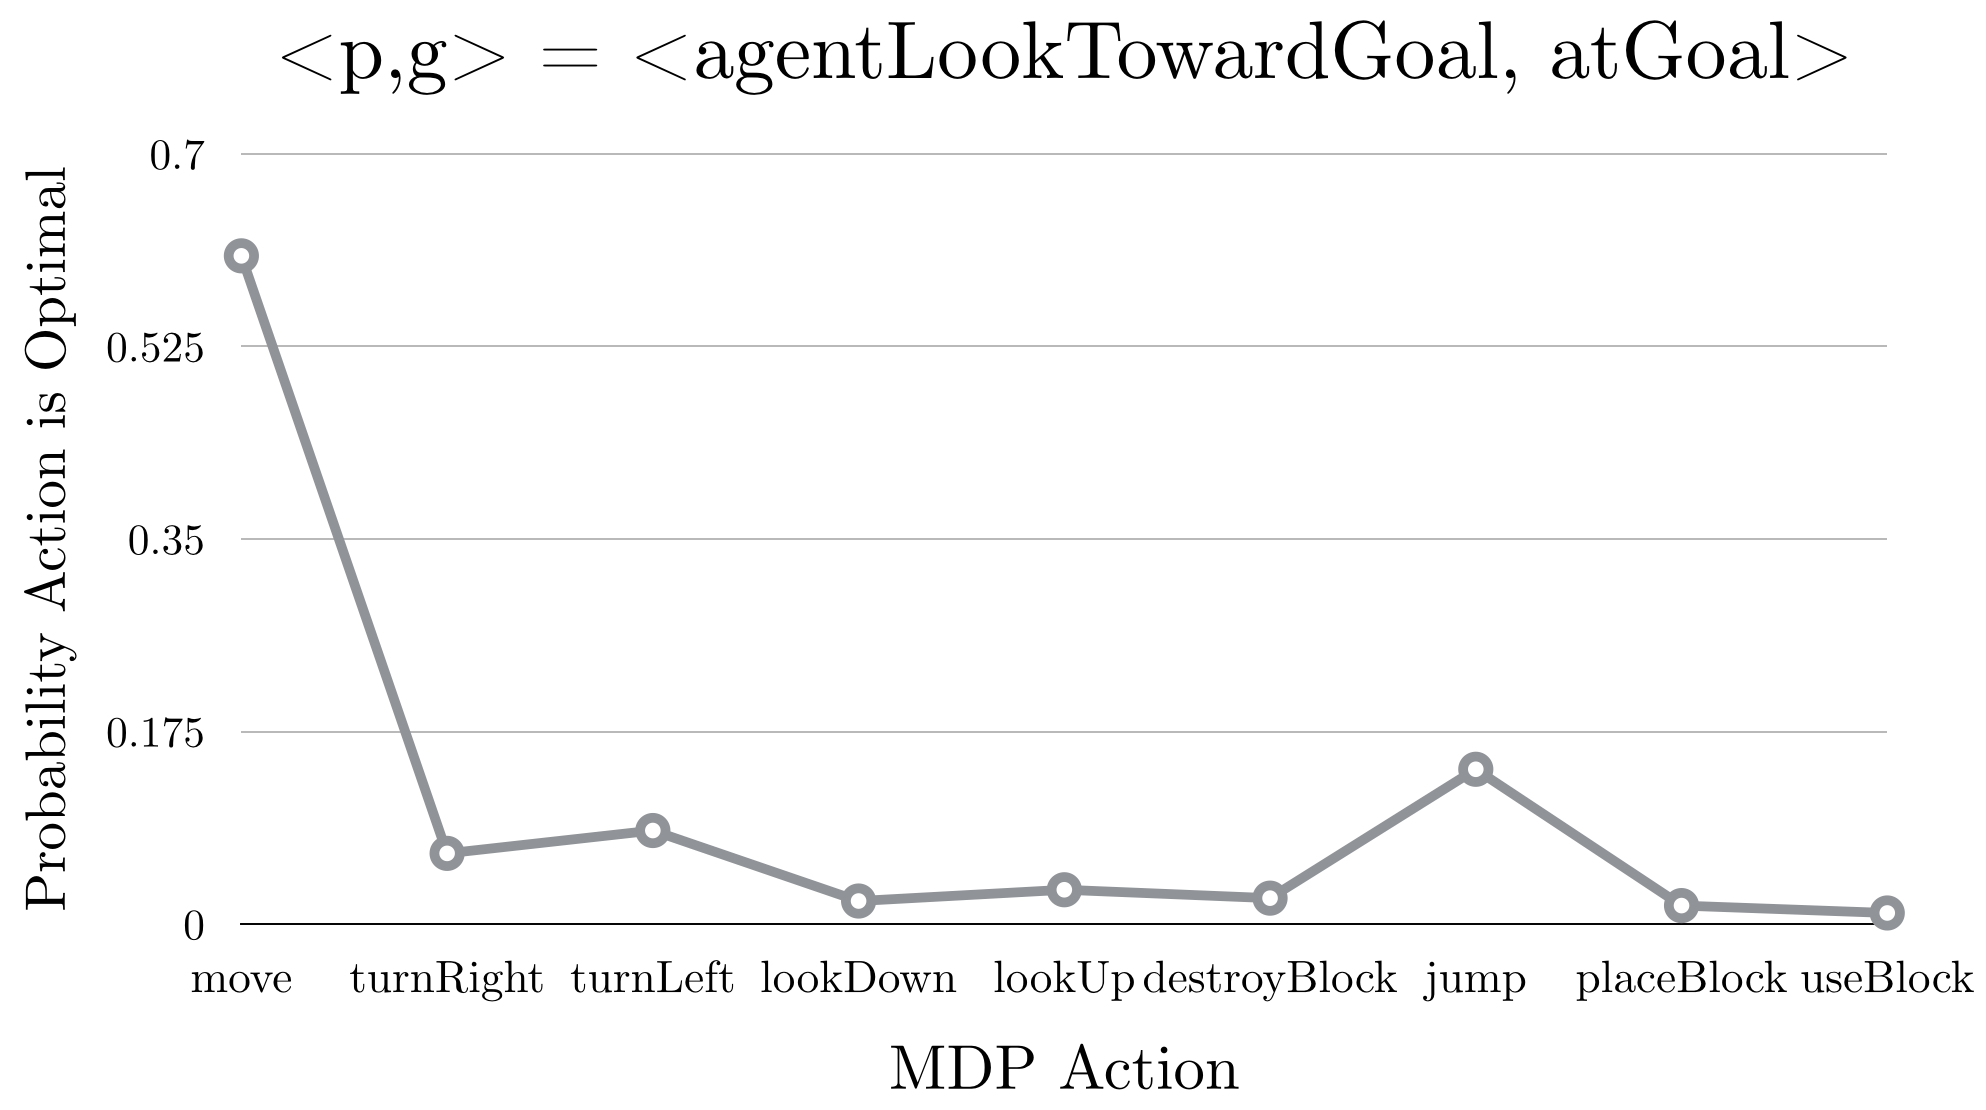
\includegraphics[scale=0.17]{figures/plane_aff.png}}
\subfigure[trenchInFrontOfAgent]{
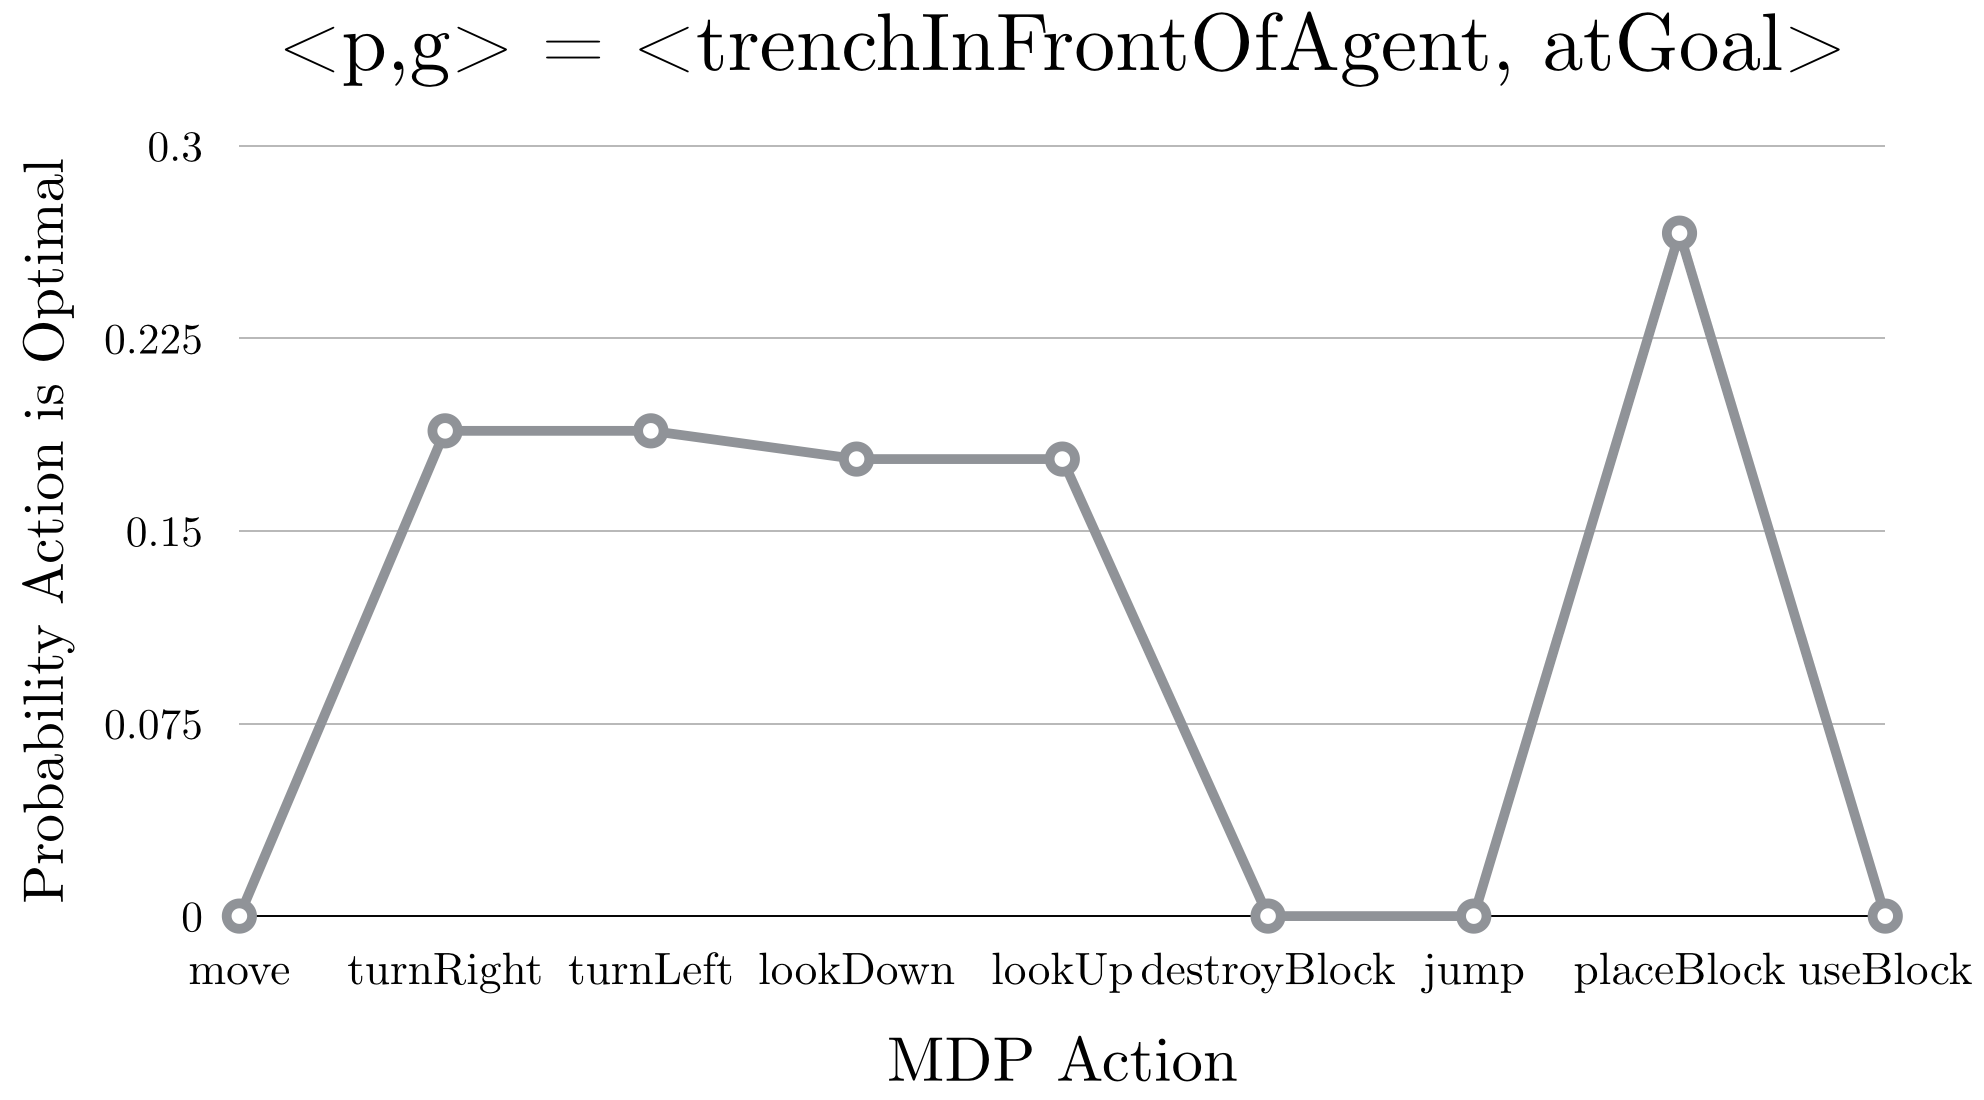
\includegraphics[scale=0.17]{figures/trench_aff.png}}
\label{fig:example_affs}
\caption{When the agent is looking toward its goal location, it is generally better to move forward than do anything else. Alternatively, when the agent is faced with a trench, the agent should walk along the trench to look for gaps, or build a bridge across by looking down and placing blocks.}
\end{figure}

At test time, the agent will see different, randomly generated worlds
from the same domain, and use the learned priors to increase its
speed at inferring a plan.  For simplicity, our learning process uses
a strict separation between training and test; after learning is
complete our model parameters remain fixed.

% -- Subsection: Action Pruning --
\subsection{Action Pruning with Goal-Based Action Priors}
\label{sec:action_pruning}
A planner using a goal-based action prior will prune actions on a state-by-state basis. 

Under the expert specified OR model, when $\Pr(a_i \in \mathcal{A}^*  \mid \phi_1, \ldots, \phi_n) = 0$
action $a_i$ is pruned from the planner's consideration. When
$\Pr(a_i \in \mathcal{A}^*  \mid \phi_1, \ldots, \phi_n) = 1$,
action $a_i$ remains in the action set to be searched by the planner.

% What to do with logreg/naive bayes



% -- EVALUATION --
\section{Evaluation}
\label{sec:evaluation}

We evaluate our approach using the game Minecraft. Minecraft is a 3-D blocks game in which the
user can place, craft, and destroy blocks of different types.
Minecraft's physics and action space allow users to create complex
systems, including logic gates and functional scientific graphing
calculators.

Minecraft serves as a model for robotic tasks such as cooking
assistance, assembling items in a factory, object retrieval, and
complex terrain traversal.  As in these tasks, the agent operates in a
very large state-action space in an uncertain environment.
Figure~\ref{fig:minecraft} shows three example scenes from Minecraft
problems that we explore.  Additionally, we used expert-provided priors to
enable a manipulator robot to infer helpful actions in response to a
person working on a kitchen task, shown in Figure~\ref{fig:baxter_results}.


\subsection{Experiments}



\subsection{Results}

% -- Table: Minecraft Naive Bayes results --
\begin{table}
\ra{1.15}
\small
\begin{tabular}{@{}llll@{}}\toprule
Planner & Bellman & Reward & CPU \\ \midrule
&\hspace{-10mm}{\it Mining Task} \\
\texttt{RTDP} & 17142.1 ($\pm$3843) 		& {\bf -6.5} ($\pm$1)  & {\bf 17.6s}   ($\pm$4) \\
\texttt{EP-RTDP} 	& 14357.4 ($\pm$3275) 		& {\bf -6.5}   ($\pm$1) & 31.9s   ($\pm$8) \\
\texttt{LP-RTDP} 	& {\bf 12664.0} ($\pm$9340) 	& -12.7 ($\pm$5) & 33.1s   ($\pm$23) \\\hline
&\hspace{-10mm}{\it Smelting Task} \\
\texttt{RTDP} 	& 30995.0 ($\pm$6730) 		& {\bf -8.6}   ($\pm$1) & 45.1s   ($\pm$14) \\
\texttt{EP-RTDP} 	& 28544.0 ($\pm$5909) 		& {\bf -8.6}   ($\pm$1) & 72.6s   ($\pm$19) \\ 
\texttt{LP-RTDP} 	& {\bf 2821.9} 	 ($\pm$662) 	& -9.8   ($\pm$2) & {\bf 7.5s}  ($\pm$2) \\ \hline
&\hspace{-10mm}{\it Wall Traversal Task} \\
\texttt{RTDP} & 45041.7 ($\pm$11816) 		& -56.0   ($\pm$51) & {\bf 68.7s}   ($\pm$22) \\
\texttt{EP-RTDP} 	& 32552.0 ($\pm$10794) 		& -34.5   ($\pm$25) & 96.5s   ($\pm$39) \\ 
\texttt{LP-RTDP} 	& {\bf 24020.8} ($\pm$9239) 	& {\bf -15.8}   ($\pm$5) & 80.5s   ($\pm$34) \\ \hline
&\hspace{-10mm}{\it Trench Traversal Task} \\
\texttt{RTDP}  	& 16183.5 ($\pm$4509) 		& {\bf -8.1}   ($\pm$2) & 53.1s   ($\pm$22) \\
\texttt{EP-RTDP} 	& {\bf 8674.8} 	($\pm$2700) 	& -8.2   ($\pm$2) & {\bf 35.9s}   ($\pm$15) \\ 
\texttt{LP-RTDP} 	& 11758.4 ($\pm$2815) 		& -8.7   ($\pm$1) & 57.9s   ($\pm$20) \\ \hline
&\hspace{-10mm}{\it Plane Traversal Task} \\
\texttt{RTDP} & 52407 ($\pm$18432) 		& -82.6   ($\pm$42) & 877.0s   ($\pm$381) \\
\texttt{EP-RTDP} 	& 32928 ($\pm$14997) 		& -44.9   ($\pm$34) & 505.3s   ($\pm$304) \\
\texttt{LP-RTDP} 	& {\bf 19090} 	 ($\pm$9158) 	& {\bf-7.8}   ($\pm$1) & {\bf 246s}  ($\pm$159) \\
\bottomrule
\end{tabular}
\caption{RTDP vs. EP-RTDP vs. LP-RTDP}
\label{table:minecraft_results}
\end{table}

Our experiments consist of five common goals in Minecraft:
bridge construction, gold smelting, tunneling through
walls, digging to find an object, and path planning.

% TRAINING
The training set consists of 20 randomly generated instances of each goal, for a total of 100 instances. Each instance is extremely simple: 1,000-10,000 states (small enough to solve with tabular approaches). The output of our training process is the model parameter $\theta$, which informs our goal-based action prior. The full training process takes approximately one hour run in parallel on a computing grid, with the majority of time devoted to computing the optimal value function for each training instance.

% TEST
The test set consists of 20 randomly generated instances of the same goal, for a total of 100 instances. Each instance is extremely complex: 50,000-1,000,000 states (which is far too large to solve with tabular approaches).


We fix the number of features at the start of training based on the number
predicates defined by the OO-MDP, $|\mathcal{P}|$, and the number of goals, $|G|$.
We provide our system with a set of 51 features that are likely to aid in predicting the correct action across instances.

We use Real-Time Dynamic Programming (RTDP)~\cite{barto95} as our
baseline planner, a sampling-based algorithm that does not require the
planner to exhaustively explore states. We compare RTDP with learned
priors RTDP (LP-RTDP), and expert priors RTDP (EP-RTDP).
We terminate each planner when the maximum change in
the value function is less than 0.01 for 100 consecutive policy
rollouts, or the planner fails to converge after 1000 rollouts.  The
reward function is $-1$ for all transitions, except transitions to
states in which the agent is in lava, where we set the reward to
$-10$. The goal specifies terminal states, and the discount factor is
$\gamma = 0.99$.  To introduce non-determinism into our problem,
movement actions (move, rotate, jump) in all experiments have a small
probability (0.05) of incorrectly applying a different movement
action.  This noise factor approximates noise faced by a physical
robot that attempts to execute actions in a real-world domain and
can affect the optimal policy due to the existence of lava pits
that the agent can fall into. 

% -- Figure: Average results --
\begin{figure}[t]
%\begin{figure}
\centering
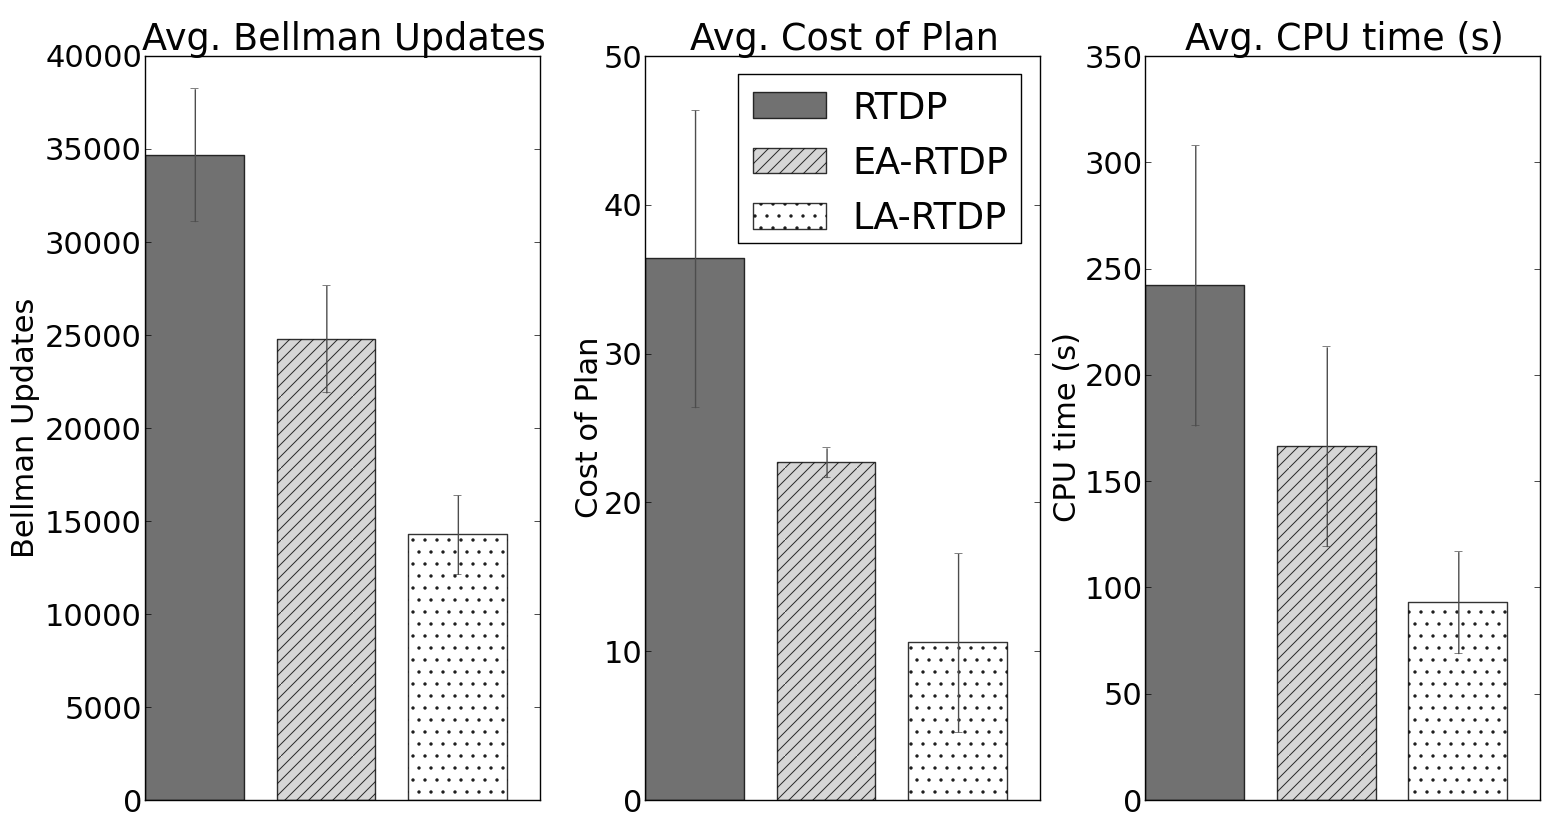
\includegraphics[width=1\linewidth]{figures/average_results_cropped.png}%
%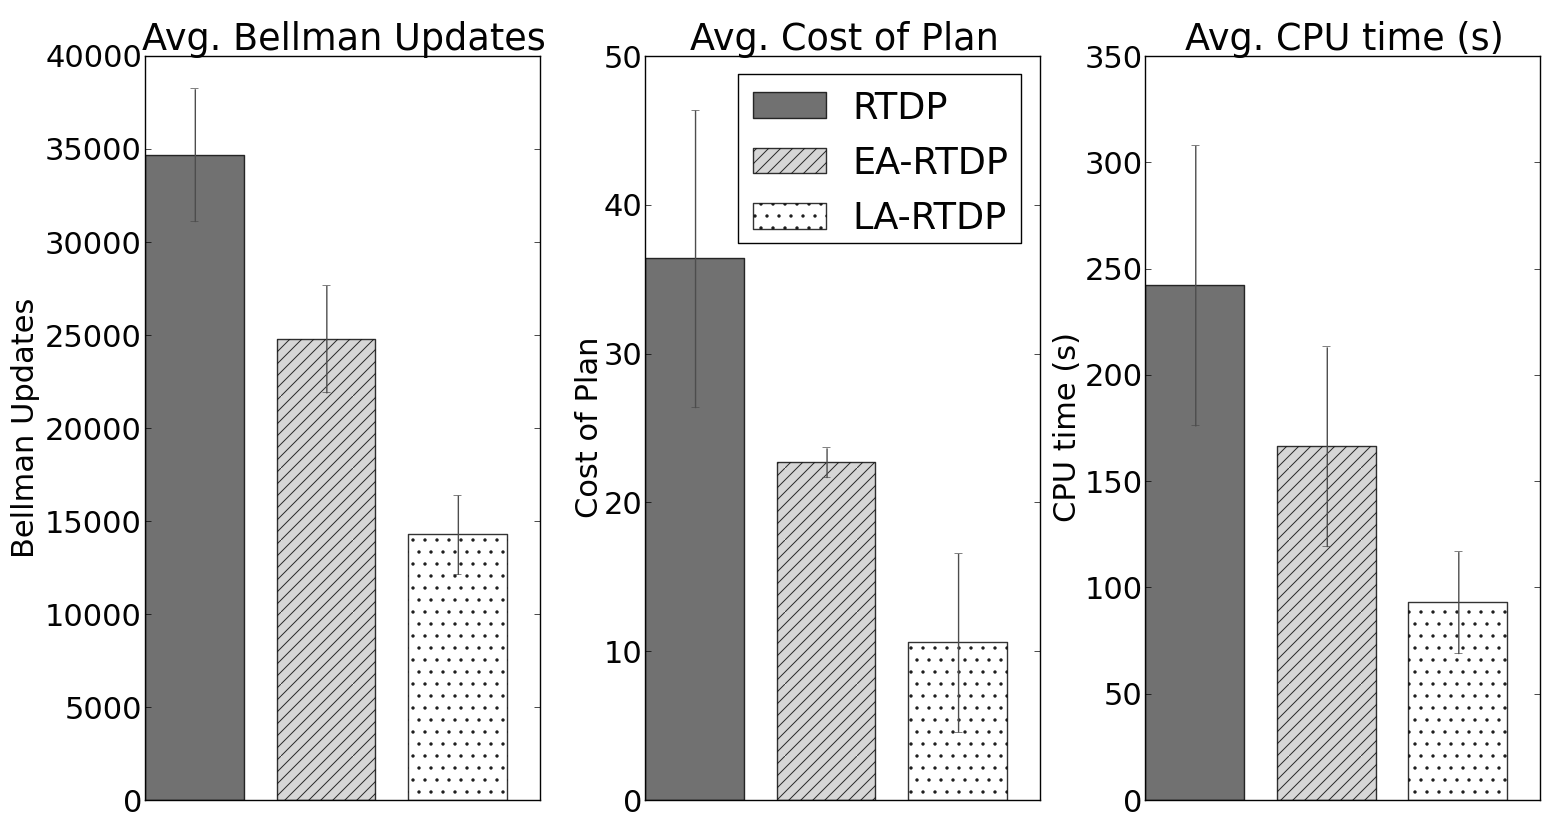
\includegraphics[scale=0.18]{figures/average_results_cropped.png}%
\caption{Average results from all maps.}
\label{fig:average_results}
\end{figure}
%\end{figure}

We report the number of Bellman updates executed by each planning
algorithm, the accumulated reward of the average plan, and the CPU
time taken to find a plan. Table~\ref{table:minecraft_results} shows
the average Bellman updates, accumulated reward, and CPU time for
RTDP, LP-RTDP and EP-RTDP after planning in 20 different maps of each
goal (100 total). Figure~\ref{fig:average_results} shows the
results averaged across all maps.  We report CPU time for
completeness, but our results were run on a networked cluster where
each node had differing computer and memory resources. As a result,
the CPU results have some variance not consistent with the number of
Bellman updates in Table~\ref{table:minecraft_results}.  Despite this
noise, overall the average CPU time shows statistically significant
improvement overall with our priors, as shown in
Figure~\ref{fig:average_results}. Furthermore, we reevaluate each
predicate every time the agent visits a state, which could be optimized by caching predicate evaluations, further
reducing the CPU time taken for EP-RTDP and LP-RTDP.

Because the planners terminate after a maximum of 1000
rollouts, they do not always converge to the optimal policy. LP-RTDP on
average finds a comparably better plan (10.6 cost) than EP-RTDP (22.7
cost) and RTDP (36.4 cost), in significantly fewer
Bellman updates (14287.5 to EP-RTDP's 24804.1 and RTDP's 34694.3), and in
less CPU time (93.1s to EP-RTDP's 166.4s and RTDP's 242.0s).  These
results indicate that while learned priors provide the largest
improvements, expert-provided priors can also significantly
enhance performance. Depending on the domain, expert-provided priors can add
significant value in making large state spaces tractable without the
overhead of supplying training worlds.

For some task types, LP-RTDP finds a slightly worse plan on average than
RTDP ({\em e.g.} the mining task). This worse convergence is due to the fact that LP-RTDP
occasionally prunes actions that are in fact optimal (such as
pruning the \texttt{destroy} action in certain states of the mining task).
%To fix this, we could lower the threshold to allow for even more conservative action pruning. In future work, we plan on investigating approaches
%to dynamically adjusting the threshold based on planning feedback. 
Additionally, RTDP occasionally achieved a faster clock time because EP-RTDP and LP-RTDP also evaluate several OO-MDP predicates in every state, adding a small amount of time to planning.





\subsection{Analysis}


% --- Conclusion ---
\section{Conclusion}

% --- Bibliography ---
\bibliographystyle{plain}
\bibliography{main}

\end{document}